% !TeX encoding = UTF-8
% !TeX TS-program = pdflatex
% !TeX spellcheck = de_DE

\def\version{\today L. Schink}
% Verlauf
% v 1.1 20.2.20202 S. Schramm - Initiale Version
% v 1.2 20.2.20202 A. Dürrbaum - Anpassungen Ttielseite / Indices

% Dokumenteneinstellung
\documentclass[a4paper,11pt,cleardoubleempty]{scrbook}

%% Einstellungsdatei
% !TeX spellcheck = de_DE

% Do's & Dont's in LaTeX
%\RequirePackage[l2tabu,orthodox]{nag}

% Deutsch und UTF-8 Encoding
\usepackage[english,ngerman]{babel}
\selectlanguage{ngerman}

\usepackage[utf8]{inputenc}
\usepackage[T1]{fontenc}
\usepackage{lmodern}

% Seiteneinstellungen
\usepackage{geometry}
\geometry{left=35mm,right=35mm, bindingoffset=0mm, top=30mm,bottom=30mm}

% Abstand im Text
\usepackage{xspace}
\usepackage{setspace}

% Kapitelüberschrift: große Nummer -> Titel
\renewcommand*{\chapterformat}{\mbox{\chapappifchapterprefix{\nobreakspace}\scalebox{3}{\thechapter}\enskip}}

% Linie unter \chapter
\makeatletter
\renewcommand{\chapterlinesformat}[3]{%
  \parbox[t]{\linewidth}{%
    \raggedchapter\@hangfrom{#2}{#3}\par%
    \vspace*{-.75\ht\strutbox}\rule{\linewidth}{.8pt}%
  }%
}
\makeatother

% pdf Pakete
\usepackage[pdfusetitle=true,colorlinks=true,linkcolor=blue,urlcolor=blue,citecolor=blue,bookmarks=true,bookmarksopenlevel=2]{hyperref}

% Pakete für Grafiken
\usepackage{graphicx}
\usepackage{color}
\usepackage{xcolor}
\usepackage{tikz}
\usepackage{pgfplots}
\pgfplotsset{compat=1.5}
\usepackage{caption}
\captionsetup{labelfont=bf, textfont=small} 
\usepackage{subcaption}

% Tabellentools
\usepackage{supertabular}
\usepackage{multirow}
\usepackage{multicol}

% Mathematik
\usepackage[fleqn]{amsmath}
\usepackage{amssymb,amsthm,textcomp}
\usepackage{upgreek}

% Zahlenformate
\usepackage{siunitx}
\sisetup{range-phrase=\ \textrm{bis}\ }
\sisetup{locale=DE}

% Auflistungen
\usepackage{enumerate}
\usepackage{enumitem}

% Symbolverzeichnis
\usepackage[nomentbl]{Einstellungen/nomencl-table}

% Glossar
%\usepackage[nonumberlist,toc,nopostdot,style=alttree,xindy]{glossaries}
\usepackage{glossaries}

% Index
\usepackage{makeidx}

% Listings
\usepackage{listings}

% Eigene Tabellenspalten
\usepackage{tabularx}
\usepackage{dcolumn}

%%%%%%%%%%%%%%%%%%%%%%%%%%%%%%%%%%%%%%%%%%%%%%%%%%%%%%%%%%%%%%%%%%%%%%%%%%%%%%
% HIER EIGENE PAKETE HINZUFÜGEN
%
%
%
%
%%%%%%%%%%%%%%%%%%%%%%%%%%%%%%%%%%%%%%%%%%%%%%%%%%%%%%%%%%%%%%%%%%%%%%%%%%%%%%
% Vor dem Laden von weiteren Paketen in das Latex-Sündenregister von Marc Ensenbach schauen!
%%%%%%%%%%%%%%%%%%%%%%%%%%%%%%%%%%%%%%%%%%%%%%%%%%%%%%%%%%%%%%%%%%%%%%%%%%%%%%

%%%%% Sonstiges
\usepackage{grffile}

% Es können todo-Notes eingefügt werden
\usepackage{todonotes}

% Definition der Kopf und Fußzeilen
\usepackage{fancyhdr,lastpage}
\fancypagestyle{fancy2}{%
	\fancyhf{}
	\fancyhead[L]{}
	\fancyhead[C]{}
	\fancyhead[R]{}
	\fancyfoot[OL]{}
	\fancyfoot[EL]{\thepage}
	\fancyfoot[C]{ }
	\fancyfoot[OR]{\thepage}
	\fancyfoot[ER]{}
	\renewcommand{\headrulewidth}{1pt}
	\renewcommand{\footrulewidth}{1pt}
}
\fancypagestyle{plain}{%
	\fancyhf{}%
	\renewcommand{\headrulewidth}{0pt}%
	\renewcommand{\footrulewidth}{0pt}
	\fancyfoot[OR]{\thepage}
}
\renewcommand{\headrulewidth}{0pt}
\renewcommand{\footrulewidth}{0pt}
\usepackage{emptypage}

% \matr{A} ergibt "fettes A" wie es bei Matrizen aussehen soll
\newcommand{\matr}[1]{\mathbf{#1}}

% Definition der Uni Kassel Farbpalette
\definecolor{UKDunkelGrau}{RGB}{87,87,87}
\definecolor{UKMittelGrau}{RGB}{157,157,157}
\definecolor{UKHellGrau}{RGB}{218,218,218}
\definecolor{UKDunkelPink}{RGB}{154,12,70}
\definecolor{UKMittelPink}{RGB}{199,16,92}
\definecolor{UKHellPink}{RGB}{243,216,221}
\definecolor{UKGruen}{RGB}{21,56,36}
\definecolor{UKBlau}{RGB}{80,149,200}
\definecolor{UKGelb}{RGB}{196,210,15}
\definecolor{UKTuerkis}{RGB}{74,172,150}
\definecolor{UKGold}{RGB}{234,195,114}

%%%%%%%%%%%%%%%%%%%%%%%%%%%%%%

\renewcommand{\familydefault}{\rmdefault}
\renewcommand*\rmdefault{ppl}

\setlength{\parindent}{0pt}
\setlength{\parskip}{6pt}

\makeatletter
% !TeX spellcheck = de_DE
\renewcommand{\maketitle}{\fontfamily{cmss}\selectfont
  \begin{center}
	\vspace*{-0.5cm}
	
\includegraphics[width=75mm]{Bilder/UniKS-Logo}\\

	\vspace{1.5cm}
	\centering
        \ifthenelse{\equal{\Typ}{MSc}}{
	% Masterarbeit
	\textbf{\Large Masterarbeit}\\[1ex]
        }{\ifthenelse{\equal{\Typ}{BSc}}{
	% Bachelorarbeit
	\textbf{\Large Bachelorarbeit}\\[1ex]
        }{
        %  Restliche Arbeiten:
	\textbf{\Large \Typ}\\[4ex]
        }}
	\textsf{\Huge \@title}\\[4ex]
%
	{\Large \@author}\\[4ex]
%
        \ifthenelse{\isundefined{\Titelgrafik}}{}{
  	  \vfill
          \includegraphics[height=8cm]{\Titelgrafik}
  	  \vfill
        }
	\vfill
        \ifthenelse{\equal{\Typ}{Technischer Bericht}}{
        Bericht-Nr. \MRTnr\\  
        }{ 
        \begin{center}
          %\fbox{\parbox{14cm}{
          \renewcommand{\arraystretch}{1.2}
		\begin{tabularx}{\columnwidth}{p{0.5\textwidth}>{\raggedleft\arraybackslash}p{0.5\textwidth}}
			Matrikelnummer: & \MatNr\\
                        \ifthenelse{\equal{\Typ}{MSc}\or\equal{\Typ}{BSc}}{
			Erstgutachter: & \Erstgutachter\\
			Zweitgutachter: & \Zweitgutachter\\}{
			Gutachter: & \Erstgutachter\\}
                        \ifthenelse{\isundefined{\Betreuer}}{}{
			Betreuer: & \Betreuer\\}
			Tag der Abgabe: & \@date\\
                        \ifthenelse{\isundefined{\MRTnr}}{}{MRT-Nr.:& \MRTnr\\}
                      \end{tabularx}%
            %          }}
                    \end{center}
        }
	\vfill
	
\includegraphics[height=12mm]{Bilder/MRT-Logo} \hfill 
\includegraphics[height=12mm]{Bilder/ISAC-Logo}
\end{center}
}


%%% Local Variables:
%%% mode: latex
%%% TeX-master: "../MRT-Bericht-2020"
%%% End:

\makeatother

\newcounter{SeitenzahlSpeicher}

%%% Local Variables:
%%% mode: latex
%%% TeX-master: "../MRT-Bericht-2020"
%%% End:


%% Alternative zu Schriftart Calibri
\usepackage[sfdefault,lf]{carlito}


%% Benötigte Daten!
\title{\fontsize{16}{14}\selectfont Implementierung einer robotergestützten Lagerverwaltung in Python\\
{\fontsize{10}{10}\selectfont Mit kameragestützen Validierungsprozessen in der Industrie 4.0-Plattform Modellfabrik $\mu$Plant}}
\date{\today}
\author{Lennart Schink}
\def\MatNr{33237484}
 
%% Wenn \geburtsort auskommentiert -> Ausgabe von
%%  Geburtsag und Geburtsort auf Deckblatt
\def\Geburtsort{Bad Bergzabern}\def\Geburtstag{31.12.1990}

%% Art des Berichtes (eines auskommentieren)
%\def\Typ{MSc}
%\def\Typ{Seminararbeit}
\def\Typ{BSc}
%\def\Typ{Seminararbeit}
%\def\Typ{Technischer Bericht}

%% MRT-Nummer, wenn schon bekannt
\def\MRTnr{N.N}

%% Auskommentieren, wenn eine Grafig auf dem Titelblatt erscheinen sollen
% maximale Höhe: 5cm, max. Breite 15 cm
%\def\Titelgrafik{Bilder/Wissenschaft.jpg}

%% Gutachter
\def\Erstgutachter{Univ.-Prof.~Dr.-Ing. Andreas Kroll}
\def\Zweitgutachter{Dr.-Ing. Robert Schmoll } % nur bei MSc oder BSc

%% Auskommentieren, wenn der/die Betreuer auf dem Titelblatt erscheinen sollen
\def\Betreuer{Dip.-Ing. Axel Dürrbaum} % Mehrer Betreuer möglich

%% PDF mit Aufgabenstellung
\def\Aufgabenstellung{Bilder/Aufgabenstellung.pdf}

%% MRT-Informationen im PDF
\pdfinfo{
   /Author \@author
   /Title \@title
   /CreationDate \@date
   /Subject \Typ
   /Keywords (MRT;LaTeX)
}


% --------------------------------------------------------------------
% Benutzerdefinierte Makros
% --------------------------------------------------------------------

% Schreibweise für Vektoren
\def\Vektor#1{\ensuremath{\mathbf{#1}}}

% Transponieren einesVektors/einer Matrix
\def\Trans#1{\ensuremath{#1^{\mathrm{T}}}}

% Variable/Zahlenwert mit Einheit
\def\Einheit#1#2{\ensuremath{#1 \text{ in } \mathrm{#2}}}

% --------------------------------------------------------------------
% Abkürzungsverzeichnis
\makeglossary
\newcommand*{\Glossar}[3]{#3 (\gls{#1})\newglossaryentry{#1}{name=#2,
    description={#3}}}

% Symbolverzeichnis
\makenomenclature
\renewcommand{\nomname}{Symbolverzeichnis}
\newcommand*{\Symbol}[2]{#1\nomenclature{#1}{#2}{}{}}
\newcommand*{\SymbolT}[2]{#2 #1\nomenclature{#1}{#2}{}{}}
\newcommand*{\SymbolE}[3]{#2 #1\nomenclature{#1}{#2}{#3}{}}
\newcommand*{\SymbolB}[4]{#2 #1\nomenclature{#1}{#2}{#3}{#4}}

% Index
\makeindex
\newcommand*{\Index}[1]{#1\index{#1}}

% --------------------------------------------------------------------
  
% Beginn des Dokuments
\begin{document}
\pagenumbering{Roman}

% Bei Problemen mit überhängenden Absätzen kann Sloppy zur Aufweichung
% der Satzparameter genutzt werden. Dies wird offiziell nicht
% empfohlen, kann aber u. U. zu guten Ergebnissen führen.
%\sloppy

% --------------------------------------------------------------------------
% Titelseite (IMMER)
% --------------------------------------------------------------------------
\fancyhf{}
\pagestyle{empty}
\maketitle 
\cleardoublepage

% --------------------------------------------------------------------------
% Aufgabenstellung (IMMER) 
% PDF-Aufgabenstellung von Betreuer geben lassen und hier einfügen
% --------------------------------------------------------------------------
\ifthenelse{\equal{\Typ}{MSc}\or\equal{\Typ}{BSc}}{
\begin{figure}[!htbp]\centering
\fbox{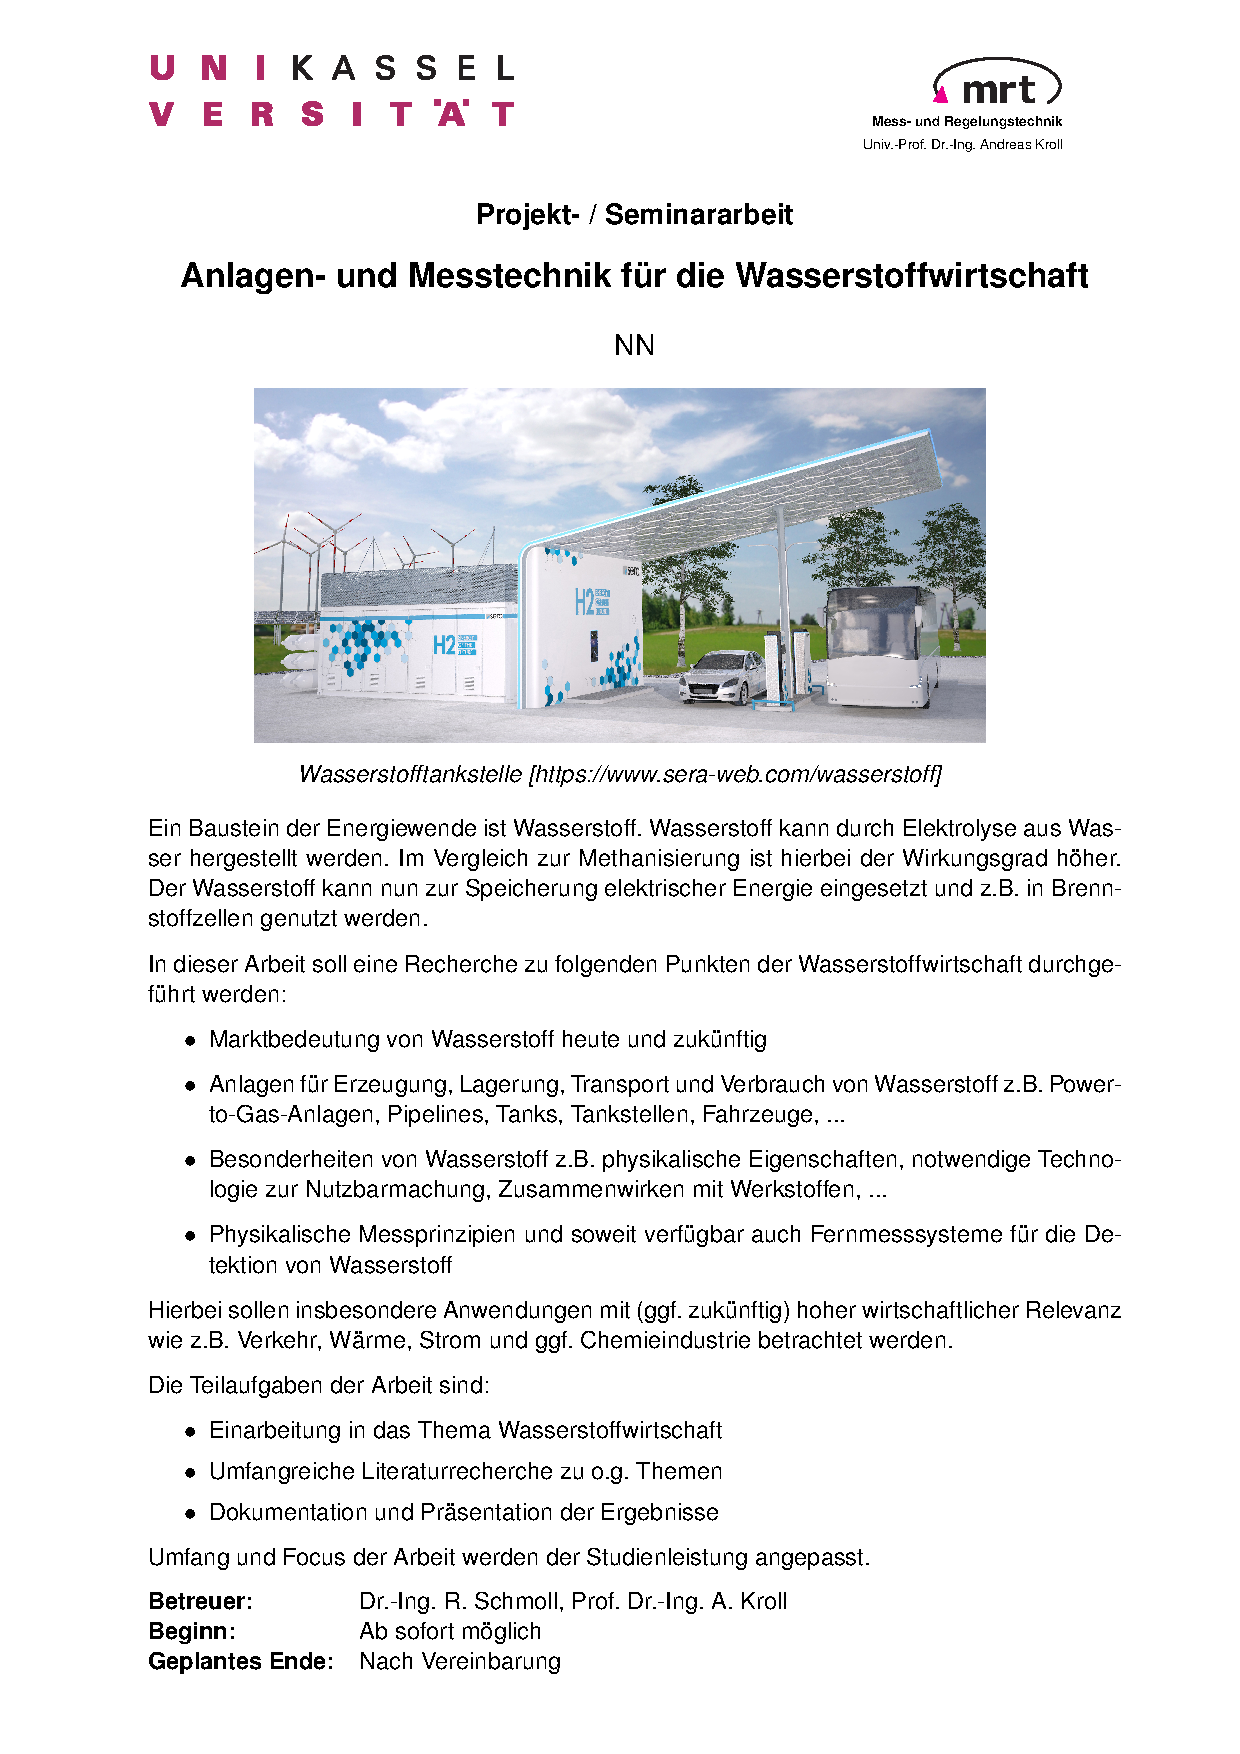
\includegraphics[width=1.0\textwidth,page=1]{\Aufgabenstellung}}
\end{figure}

\begin{figure}[!htbp]
\centering
\fbox{\includegraphics[width=1.0\textwidth,page=2]{\Aufgabenstellung}}
\end{figure}
\cleardoublepage
}{}

% --------------------------------------------------------------------------
% Versicherung (BEI BA UND MA)
% --------------------------------------------------------------------------
\ifthenelse{\equal{\Typ}{MSc}\or\equal{\Typ}{BSc}}{
% !TeX encoding = UTF-8
% !TeX TS-program = pdflatex
% !TeX spellcheck = de_DE

\chapter*{Versicherung}

Hiermit versichere ich, dass ich die vorliegende Arbeit selbstständig
verfasst und keine anderen als die angegebenen Quellen und Hilfsmittel
verwendet habe.

\vspace*{5ex}
\rule{12cm}{0.5pt}\newline
Ort, Datum, Unterschrift


%%% Local Variables:
%%% mode: latex
%%% TeX-master: "../MRT-Bericht2020"
%%% End:

\cleardoublepage
}{}

% --------------------------------------------------------------------------
% Zusammenfassung (BEI BA UND MA)
% --------------------------------------------------------------------------
\ifthenelse{\equal{\Typ}{MSc}\or\equal{\Typ}{BSc}}{
% !TeX spellcheck = de_DE
\chapter*{Kurzfassung}

Diese Bachelorarbeit widmet sich der Untersuchung des Einsatzes optischer Marker zur Verbesserung von Inventurprozessen in automatischen Lagerzellen. 
Die Arbeit stützt sich auf Erkenntnisse aus den Arbeiten von \cite[Hübler (2019)]{Hübler2019} und \cite[Kistner (2017)]{LarsKistner2017}  auf
und nutzt zwei Kameras zur Markererkennung: Eine Übersichtskamera in der oberen Ecke der Lagerzelle und eine Kamera, die am Greifer angebracht ist.

Die Implementierung der Inventurprozesse erfolgt in der Warehouse Management Software, wobei Python 3.11 im Backend und das Qt Framework mit PySide6 Bindings 
im Frontend verwendet werden. 
Die Bildverarbeitung und Markererkennung erfolgt mithilfe der Open-Source-Bibliothek OpenCV, und die perspektivische 
Entzerrung wird mit scikit-image durchgeführt.

Im Vorfeld dieser Arbeit wurden umfangreiche Vorarbeiten im Rahmen meiner \cite[Semesterarbeit]{Semesterarbeit} geleistet, 
darunter die Erarbeitung einer Softwarearchitektur für die bestehende Lagerverwaltungssoftware Lagerverwaltung 3.0 (Rodriguez, 2019) 
sowie Überlegungen zur Auswahl der Kameras. Anlass zur Neuimplementierung der Lagerverwaltungssoftware ist der Wunsch einer 
eiheitlichen Programmiersprache in der Modellfabrik $\mu$Plant und der Wechsel des Betriebssystems von Windows 7 auf Windows 10.
Die ursprüngliche Implementierung in C$\#$ funktioniert nicht mehr fehlerfrei unter Windows 10.
Außerdem baut die alte Implementierung auf dem Protokoll Modbus auf, das in der $\mu$Plant durch den Industriestandard OPC UA ersetzt wird.

Die Arbeit beinhaltet viele Aspekte der modernen Softwareentwicklung, einschließlich der Implementierung von Plug-Ins, 
Integration von Legacy-Schnittstellen, portierung der M2M-Kommunikation von Modbus nach OPC UA und eine Forschungskomponente z
ur arUco Marker-Erkennung. 

Abschließend werden eigene Überlegungen zur grundsätzlichen Erkennung der Behälter präsentiert, 
die als Anregung für zukünftige Forschungsarbeiten dienen sollen.

\ifthenelse{\equal{\Typ}{MSc}}{
\vfill
\section*{Summary}
\begin{otherlanguage}{english}
Awaken the reader's interest here!

Why should he read this - exactly this - work?
\end{otherlanguage}

\selectlanguage{ngerman}
}{}

%%% Local Variables:
%%% mode: latex
%%% TeX-master: "../MRT-Bericht-2020"
%%% End:

\cleardoublepage
}{}

% --------------------------------------------------------------------------
% Summary (BEI MA)
% --------------------------------------------------------------------------
%\ifthenelse{\equal{\Typ}{MSc}}{
%\include{Kapitel/Summary}
%\cleardoublepage
%}{}

% --------------------------------------------------------------------------
% Inhaltsverzeichnis (IMMER)
% --------------------------------------------------------------------------
\tableofcontents
\cleardoublepage

% --------------------------------------------------------------------------
% Liste der Tabellen und Bilder und Listings
% --------------------------------------------------------------------------
\listoftables      % optional
\listoffigures     % optional
\lstlistoflistings % optional
\cleardoublepage

% --------------------------------------------------------------------------
% Abkürzungsverzeichnis (IMMER)
% --------------------------------------------------------------------------
% !TeX spellcheck = de_DE
\chapter*{Abkürzungsverzeichnis}
\addcontentsline{toc}{chapter}{Abkürzungsverzeichnis}

\begin{center}
	
	\renewcommand{\arraystretch}{1.1}
	\tablefirsthead{\hline \textbf{Abkürzung} & \textbf{Bedeutung} \\ \hline}
	\tablehead{\hline \textbf{Abkürzung} & \textbf{Bedeutung} \\ \hline}
	
	\begin{supertabular}{p{2.1cm}p{10.9cm}}
		GUI				& \textbf{G}raphical \textbf{U}ser \textbf{I}nterface \\
		UML				& \textbf{U}nified \textbf{M}odeling \textbf{L}anguage \\
		MES				& \textbf{M}anufacturing \textbf{E}xecuting \textbf{S}ystem\\
		C\#				& An object oriented, component oriented programming language\\
		C++				& A high level, general purpose programming language\\
		QML				& \textbf{Q}t-Project's Interface \textbf{M}arkup \textbf{L}anguage\\
		LZ				& \textbf{L}ager\textbf{zelle} der $\mu$Plant\\
		FZ				& \textbf{F}ertigungs\textbf{zelle} der $\mu$Plant \\
		AuE				& \textbf{A}bfüll- \textbf{u}nd \textbf{E}ntleer - Station der $\mu$Plant \\
		RFID			& \textbf{R}adio \textbf{F}requency \textbf{ID}entification\\
		TCP/IP			& \textbf{T}ransmission \textbf{C}ontrol \textbf{P}rotocoll / \textbf{I}nternet \textbf{P}rotocoll\\
		MVC				& \textbf{M}odel - \textbf{V}iew - \textbf{C}ontroller, Ein Design-Konzept für Software\\
		URI				& \textbf{U}niform \textbf{R}essource \textbf{I}dentifier, Im Qt Framework kann dies eine beliebige
						  Ressource sein. Z.B. eine URL, ein Bild oder ein Programmteil. \\
		QML Type		& Ein QML Basiselement. Enthält alle für die Visualisierung nötigen Attribute. Eine Liste
						  aller QML Types findet sich hier \cite{qmlTypeList}\\
		RAPID			& Eine speziell für die Robotersteuerung entwickelte Programmiersprache\\
		RST				& \textbf{R}e\textbf{s}tructured \textbf{T}ext Eine einfache markup language die in Sphinx benutzt wird\\
	\end{supertabular}

\end{center}
\addcontentsline{toc}{chapter}{Abkürzungsverzeichnis}
\printglossary[title={Abkürzungsverzeichnis},toctitle={Abkürzungsverzeichnis}]
\cleardoublepage

% --------------------------------------------------------------------------
% Symbolverzeichnis (IMMER)
% --------------------------------------------------------------------------
%% !TeX spellcheck = de_DE
\chapter*{Symbolverzeichnis}
\addcontentsline{toc}{chapter}{Symbolverzeichnis}

\begin{center}
	
	\renewcommand{\arraystretch}{1.1}
	\tablefirsthead{\hline \textbf{Symbol} & \textbf{Beschreibung} & \textbf{Einheit} \\ \hline}
	\tablehead{\hline \textbf{Symbol} & \textbf{Beschreibung} & \textbf{Einheit} \\ \hline}
	
	\begin{supertabular}{p{1.85cm}p{9cm}p{1.85cm}} % GESAMT 12.7cm!
		% Latein: Alphabetisch + 1. Matrizen, 2. Großbuchstaben, 3. Vektoren, 4. Kleinbuchstaben
		$\varepsilon$ 	& Emissionsgrad 	& - \\
	\end{supertabular}

\end{center}
\addcontentsline{toc}{chapter}{Symbolverzeichnis}
\printnomenclature
\cleardoublepage

% --------------------------------------------------------------------------
% Index (optional)
% --------------------------------------------------------------------------
\addcontentsline{toc}{chapter}{Index}
\printindex
\cleardoublepage


% --------------------------------------------------------------------------
% Hauptteil der Arbeit (IMMER)
% --------------------------------------------------------------------------
\pagestyle{fancy2}
\setcounter{SeitenzahlSpeicher}{\value{page}}
\pagenumbering{arabic}

% Erklärung gemäß Prüfungsordnung
% Danksagung

% !TeX encoding = UTF-8
% !TeX TS-program = pdflatex
% !TeX spellcheck = de_DE

\chapter{Motivation und Zielsetzung}

    Das Institut für Mess- und Regelungstechnik an der Universität Kassel hat in den letzten Jahren eine Modellfabrik $\mu$Plant gebaut.
    Aus über 70 Einzelarbeiten ist ein modernes Industrie-4.0 Konzept geschaffen worden.
    Teil der $\mu$Plant ist ein vollautomatisiertes Lager.
    Das Lager besteht aus einem abgetrennten Raum, dessen Zugang über eine Tür mit einem Türschalter überwacht ist.
    In diesen Bereich können autonome mobile Roboter (Turtlebots) einfahren.
    In dem abgetrennten Bereich steht ein Industrieroboter Typ ABB IRB 140 und ein Lagerregal mit ausgewiesenen 18 Lagerplätzen.
    Außerdem befindet sich neben einer Andockstation für den Turtlebot ein Kommissioniertisch. \\

    Ein pneumatischer Greifer kann Paletten, die je mit bis zu zwei Bechern bestückt werden können,
    zwischen dem mobilen Roboter und dem Lagerregal transportieren.
    Von einem PC-Arbeitsplatz aus können mittels Software die Lagerprozesse überwacht werden.
    Im Fehlerfall kann eingeschritten werden oder es können manuell Prozesse ausgelöst werden.\\

    Die Software ist derzeit in 3 Programme aufgeteilt: Einerseits gibt es die Lagerverwaltung 3.0 - die Hauptsoftware.
    Sie bildet die automatisierten Prozesse ab und verfügt über ein GUI welches u.A.\ den Bestand visualisiert.
    Daneben gibt es den Warehouse Controller, der dazu verwendet wird, manuelle Prozesse auszulösen.
    Zudem gibt es ein Programm \glqq RFID-Server\grqq mit dem über RFID Leser der Fa. Feig Tags der Transportbehälter
    ausgelesen werden können.
    \\
    Mit dem Wechsel des Betriebssystems von Windows 7 auf Windows 10 ist die Kompatibilität der C\# Implementierung
    nicht mehr gegeben.
    Außerdem laufen Teilfunktionen des Programms nicht fehlerfrei oder tolerieren kaum Fehlbedienungen.
    Die Dreiteilung der Software ist im Allgemeinen auch nicht mehr erwünscht. \\

    Diese Seminararbeit beschäftigt sich mit der Analyse der bestehenden Software:
    Es wird ermittelt, aus welchen Programmteilen und Funktionen die Software besteht.
    Aus den Erkenntnissen wird ein Konzept entwickelt, welches die Funktionen der Drei Software Teile zusammenführt.
    Dies soll die Grundlage für eine Migration der Software nach Python schaffen.

    Erkenntnisse aus der studentischen Arbeit von Sebastian Hübler aus dem Jahr 2019 \cite{Hübler2019} sollen überprüft
    und vertieft werden um Anforderungen an Kameras und arUco Marker zu ermitteln, die später eine automatisierte
    Inventur ermöglichen sollen.

    Grundlage für die Portierung und das Refactoring der Software in der Lagerzelle ist die Arbeit von \cite{LarsKistner2017}.
    In ihr sind wichtige Grundlagen zum Aufbau und zur Kommunikation der muPlant beschrieben. Unter Anderem auch das Agentensystem, welches festlegt wie die M2M-Kommunikation abläuft.

    Die C\# Programme von Rodriguez liefern wichtige Hinweise zu Programmfunktionen und ihre Implementierung. 
    Der Aufbau der Software ist in meiner Seminararbeit beschrieben. 


\cleardoublepage

\chapter{Grundlagen}

In diesem Kapitel werden die theoretischen Grundlagen für diese Arbeit aufgezeigt und Beschrieben. 

\section{arUco Marker}\label{arucoMarker}

arUco Marker sind quadratische synthetische Marker, bestehend aus einem schwarzen Rand und einer binären Matrix. Die Kantenlänge der quadratischen Elemente der Binärmatrix ist proportional zu der Dicke des schwarzen Rands. Die binäre Matrix selbst dekodiert und
als ID genutzt werden. Dabei wird die Binärmatrix jedoch nicht direkt als Binärzahl dekodiert, sondern die Marker sind ihrem Platz im Dictionary ihres Typs aufsteigend zugeordnet.
Der Erkennungs-Algorithmus nutzt Graustufenbilder und gilt als robust. 
Er beruht zunächst auf der Erkennung rechteckiger Merkmale. 
Die detektierten Bildbereiche werden anschließend in ein binäres Bild transformiert und perspektivisch entzerrt. 
Anschließend werden die Marker mit einer vordefinierten Maske dekodiert.
Die Größe der Matrix wird dabei aus dem Marker-Typ und der Breite des schwarzen Rands berechnet.
Im Standardfall entspricht die Breite des Rands genau einer Pixelbreite und -Höhe eines Bits. 
Neben der ID werden dabei auch die Ecken der Marker erkannt und die Lage im Originalbild gespeichert. 
IDs und Marker-Ecken sind die wichtigsten Rückgabewerte des Algorithmus.
Merkmale im Bild, die im Verlauf der Algorithmus als Marker abgelehnt werden, lassen sich als dritter Rückgabewert ausgeben.
Im Quellcode der Anwendung sind die Rückgabewerte stets als \verb|ids|, \verb|corners| und \verb|rejected| bezeichnet.

Durch die Lokalisierung der Ecken im Originalbild können arUco Marker gut für Aufgaben wie Kamerakalibrierung, Objektlokalisierung, Abstandsmessung sowie Roboternavigation genutzt werden.
\cite[OpenCV arUco]{OpenCVaruco}
Durch die vorgefertigte Maske ist die Erkennung immer an ein Dictionary des verwendeten Markers gebunden. 
Wichtigstes Merkmal ist dabei die Größe der Binärmatrix. In dieser Arbeit werden Marker des Typs 6x6-250 verwendet.
Dabei steht 6x6 für die Größe der Binärmatrix in Bits und 250 steht für die Anzahl der Pixel.

\begin{figure}
    \caption{Beispiel für eine erfolgreiche Erkennung von arUco Markern. Quelle: \cite[OpenCV]{OpenCVaruco}}\label{fig:aruco1}
    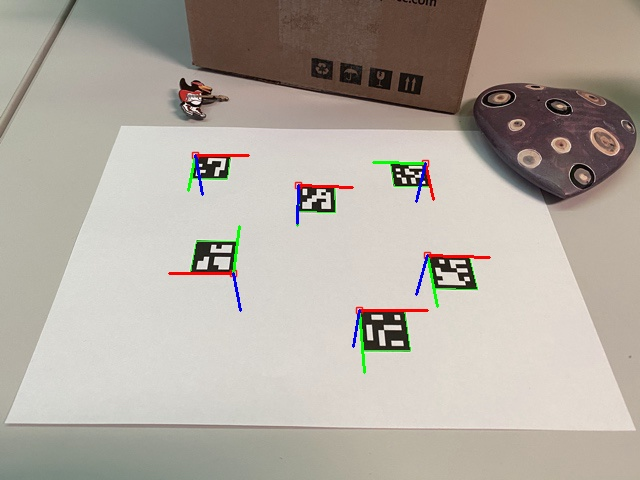
\includegraphics[width = \textwidth/2]{Bilder/singlemarkersaxes.jpg}
    \centering
\end{figure}

\begin{figure}
    \caption{Bild nach Graustufenumwandlung und Umwandlung in Binärbild. Quelle: \cite[OpenCV]{OpenCVaruco}}\label{fig:aruco2}
    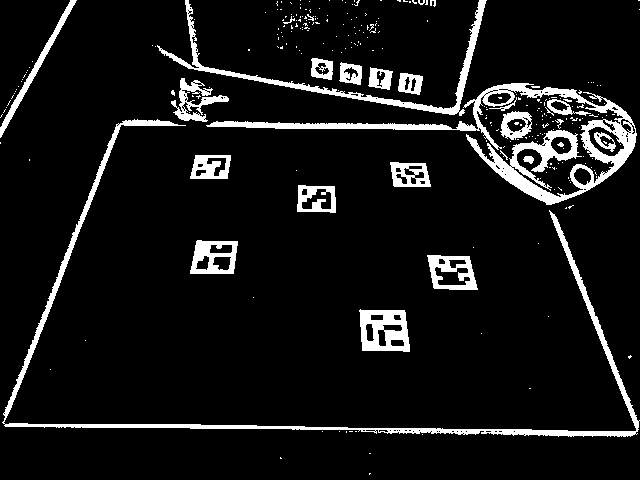
\includegraphics[width = \textwidth /2]{Bilder/singlemarkersthresh.png}
    \centering
\end{figure}

\subsection{Erkennungsalgorhitmus}
Die Erkennung der Marker erfolgt in den nachfolgenden Schritten: 

\begin{enumerate}
    \item Einlesen des Bildes, z.B. \ref{fig:aruco1}
    \item Umwandeln des Bilds in ein Graustufenbild 
    \item Umwandeln des Bilds in ein Binärbild \ref{fig:aruco2}
    \item Erkennen rechteckiger Merkmale
    \item Rektifizierung der Merkmale \ref{fig:aruco4}
    \item Bitextraktion der Binärmatrix (Bilder \ref{fig:aruco5} \ref{fig:aruco6})
    \item Decodierung der Binärmatrix ergibt die ID und Ecken des Markers
\end{enumerate}

Bei der Umwandlung in ein Binärbild kann der Erkennungsalgorithmus schon fehlschlagen. Die Gründe dafür werden im Kapitel \ref{KameragestützteInventur}
behandelt.

\begin{figure}
    \caption{Beispiel für eine fehlgeschlagene Umwandlung in ein Binärbild. Dieser Marker würde nicht erkannt. Quelle: \cite[OpenCV]{OpenCVaruco}}\label{fig:aruco3}
    
\includegraphics[width = \textwidth/2]{Bilder/singlemarkersbrokenthresh.png}
    \centering
\end{figure}

Anschließend werden rechteckige Merkmale gesucht und diese Rektifiziert \ref{fig:aruco4}. 

\begin{figure}
    \caption{Rektifizierung eines extrahierten Markers. Quelle: \cite[OpenCV]{OpenCVaruco}}\label{fig:aruco4}
    
\includegraphics[width = \textwidth/3]{Bilder/removeperspective.jpg}
    \centering
\end{figure}

\begin{figure}
    \caption{Bitextraktion der Binärmatrix. Quelle: \cite[OpenCV]{OpenCVaruco}}\label{fig:aruco5}
    
\includegraphics{Bilder/bitsextraction1.png}
    \centering
\end{figure}

\begin{figure}
    \caption{Bitextraktion der Binärmatrix. Quelle: \cite[OpenCV]{OpenCVaruco}}\label{fig:aruco6}
    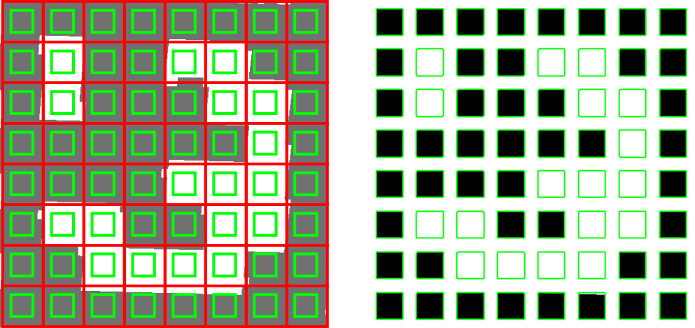
\includegraphics[width = \textwidth]{Bilder/bitsextraction2.png}
    \centering
\end{figure}



\section{Grundlagen der Softwarearchitektur}

Die in dieser Arbeit verwendeten Grundlagen zur Softwarearchitektur beschränken sich auf den Kurs "Programmierung und Modellierung" des Fachbereichs
FB16 der Universität Kassel. Der Inhalt reicht von dem Erstellen von textuellen Szenarien einer Anwendung, über die Konzeptionierung von GUIs bis hin
zu den Grundlagen der Servertechnik am Beispiel des REST-Protokolls und Websockets. 
Der größte Thementeil ist jedoch die Modellierung von Datenmodellen und ihre referenzielle Integrität, welches im Zusammenhang mit UML-Diagrammen gelernt wurde.
Referenzielle Integrität von Datenmodellen spielt in Python eine eher untergeordnete Rolle, da es keine privaten oder geschützten Klassen-Attribute gibt. 
Dennoch bietet ihre Verwendung eine gute Möglichkeit, um die Datenmodelle in ihrer gewohnten Komplexität zu gestalten, die
Verwendung jedoch einfach zu halten.

\section{OPC UA}

OPC UA ist ein offener Standard für die Kommunikation zwischen Maschinen der \cite[OPC Foundation]{OPCFoundation}. Es ist ein schlankes Protokoll, 
welches eine verschlüsselte Übermittlung von Maschineninformationen, Sensordaten, Prozessdaten und anderen Daten ermöglicht.
OPC UA ist ein wichtiger Bestandteil des Programms Industrie 4.0. 
Üblicherweise sind alle Ebenen Prozessteuerungspyramide eingebunden, die von SPSen bis hin zur Geschäftsleitung reichen kann.

Für diese Arbeit gibt es im Wesentlichen zwei Möglichkeiten das OPC UA Protokoll zu benutzen. 
Zum Einen bietet das \cite[Qt Framework]{QtOPCUA} eine Implementierung des Protokolls. 
Zum anderen gibt es ein offenes GitHub Repository \cite[FreeOpcUa]{asyncua}, das als Python Paket zur Verfügung steht. 
Da in anderen Software-Anwendungen der $\mu$Plant bereits FreeOpcUa verwendet wird, fällt die Wahl auf diese Bibliothek.
Das erleichtert die Integration der OPC UA Funktionalität in die $\mu$Plant und eine zukünftige Wartung und Erweiterung der Anwendung.

Während der Entwicklung der Anwendung wurden zu Testzwecken zwei Programme verwendet, um die erstellten Server zu testen. 
Für Windows wurde der \cite[OPC UA Client UaExpert]{UaExpert}verwendet. Da ich jedoch unterwegs auf MacOS programmiere, wurde 
ein OPC UA Client \cite[OPC UA Client für Mac]{uaClientMac} verwendet. 
Dieser hat zwar nicht den gleichen Funktionsumfang, ist aber dennoch für Debug-Zwecke nützlich. 

\section{RFID Technologie}

Laut der Website \cite[RFID Grundlagen]{RFIDGrundlagen} sind die Anfänge der RFID Technologie bis in den zweiten Weltkrieg zurückzuführen, 
in dem eine Art Sekundärradar zur Feinerkennung eingesetzt wurde. Als Begründer der heutigen RFID-Technologie gilt der Schwede Harry Stockman. 
Bei der Technologie handelt es sich um ein System zur Kontaktlosen Informationsübermittlung (Lesen und Schreiben). 
Dazu wird in der Regel ein Transponder und ein Lesegerät benötigt. Beide Einheiten fügen über ausgeprägte Antennen.
Das Lesegerät erzeugt ein elektromagnetisches Feld, welches einerseits zur Spannungsversorgung des IC des Transponders genutzt wird.
Gleichzeitig dient das Feld als Taktgeber und zur Informationsübermittlung. 
Während das Lesegerät nicht sendet, kann der Transponder Daten übermitteln. 
Für die Transponder gibt es verschiedene Standards, auf die im Rahmen dieser Arbeit nicht weiter eingegangen werden. 
Die Daten auf dem Transponder sind in Blöcke aufgeteilt, die jeweils eine bestimmte Anzahl an Bytes enthalten.
Je Transponder ist ein Block für eine UID reserviert, die im Allgemeinen nicht verändert werden kann.

In der $\mu$Plant werden Lesegeräte der Firma \cite[FEIG GmbH]{RFIDFeig} vom Typ ID ISC.MRU102-PoE-LED verwendet. 
Die Lesegeräte sind in jeder Station der $\mu$Plant verbaut.
Die Transponder sind jeweils auf der Rückseite eines jeden Bechers aufgeklebt. 
Jedem Becher ist somit eine eigene UID zugeordnet. Die Datenübertragung der Lesegeräte erfolgt über TCP/IP.
Die Firma Feig stellt ein umfassendes SDK zur Verfügung, bietet jedoch keinen Python Support.


\section{Die Programmiersprache Python}

Python ist eine universelle, interpretierte Hochsprache. Der Programmcode kommt dabei ohne Klammer und Semikolons aus.
Die Formatierung des Codes erfolgt über Einrückungen. \cite[Python]{Python} ist leicht zu lernen, intuitiv zu nutzen und unterstützt die 
meisten Programmier-Paradigmen wie objektorientierte, funktionale und aspektorientierte Programmierung. 

In dieser Arbeit wird Python 3.11 verwendet. 

\section{Die Programmiersprache C++}

C++ ist eine universelle, kompilierte Hochsprache. Sie ist eine Weiterentwicklung der Programmiersprache C und unterstützt die
Programmier-Paradigmen der Objektorientierung, generische Programmierung und prozedurale Programmierung.
Der Standard ist sehr komplex und besteht aus mehreren Teilen, die an und für sich eigenständig anwendbar, aber auch kombinierbar sind.

In dieser Arbeit wird C++ in der Version 23 verwendet, um das SDK der Firma Feig zu nutzen und ausschließlich die gewünschten Funktionen 
in Python einzubinden.

Auch für das Legacy Framework ABB Robotics wird C++ verwendet, um das Framework in Python einzubinden.
Die Programme sind dabei in Visual Studio 2019 erstellt und kompiliert worden. 

\section{Die Programmiersprache C\#}\label{Csharp}

C$\#$ ist eine Komponentenorientierte Programmiersprache und historisch die Antwort auf die, von SUN veröffentlichte, Programmiersprache Java. 
Sie wird häufig mit dem .NET Framework verwendet - so auch in der Software Lagerverwaltung 3.0, welche in meiner \cite[Semesterarbeit]{Semesterarbeit}
Grundlage für die Konzeptionierung der neuen Lager-Verwaltungs-Software war. 
Das GUI wird dabei in .xaml Dateien gespeichert, die mit einem Integrierten Editor aus der Visual Studio IDE. Der Controllercode für die GUI-Elemente 
findet sich in einer xaml.cs Datei, welche in C$\#$ implementiert sind.
Dazu gibt es in der Regel beliebig viele Dateien, die den Code für die Geschäftslogik implementieren. Der Quellcode einer solchen Anwendung is oft nicht leicht zu überschauen. 
Daher sind Teile der Anwendung Lagerverwaltung 3.0 in dieser Arbeit nur prinzipiell unter visuellen (GUI) und funktionellen Aspekten übernommen worden.

\section{Das Qt Framework}

Laut der \cite[Qt Wiki Website]{qtWikiHistory} wurde das Qt Framework geboren, als ihre Schöpfer Haa-
vard Nord und Eric Chambe-Eng im Sommer 1990 in Norwegen an einem GUI für eine
Ultraschalldatenbank arbeiteten. Die Software sollte damals in C++ implementiert auf
Mac, Unix und Windows laufen. Fünf Jahre später veröffentlichten Sie das erste Qt Fra-
mework unter dem Firmennamen Troll Tech. Seitdem gewann das Framework immer
mehr Popularität. Im Jahr 2006 übernahm Nokia die Firma Troll Tech und verkaufte das
Qt Project in den Jahren 2011 und 2012 erst teilweise, dann vollständig an den Digia
Konzern. Seit 2014 ist Qt als Tochterunternehmen des Digia Konzerns unter dem Namen
„The Qt Company“ ein eigenständiges Unternehmen.
Das Qt Framework ist in C++ implementiert.

\subsection{PySide6 Bindings}

Für die Programmiersprache wurden historisch zwei Frameworks veröffentlicht. Die Firma Riverbank veröffentlichte für das Qt4 die Bindings PyQt4.
Die Bindings sind sehr eng an der C++ Implementierung des Qt Frameworks orientiert.
Die Firma Nokia hat parallel die PySide Bindings veröffentlicht, die mehr an dem Python Syntax orientiert sind.
The Qt Company hat das PySide Framework übernommen und weiterentwickelt. 
Beide Frameworks sind sowohl mit kommerziellen als auch mit Open Source Lizenzen verfügbar.
Im Jahr 2023 wurde das PySide6 Framework für Qt6 veröffentlicht welches auch QtQuick und QML voll unterstützt. 
Bei dem PySide6 Framework handelt es sich um automatisch generierte Bindings für das Qt Framework. 
Das Qt Framework in der C++ Implementierung muss dabei immer mit installiert werden. 
Leider sind bei der automatischen Generierung der Bindings keine Dokumentationen entstanden.
Eine dauernde, parallele Recherche in der Qt Dokumentation ist daher unerlässlich und verleitet dazu eine gleichartige
Programmierweise zu entwickeln und sich auf bekannte Strukturen zu verlassen.

\subsection{QtQuick 2.0 und QML}

Neben der herkömmlichen Entwicklung für GUIS mittels Widgets,  bietet das Qt Framework auch die Möglichkeit, GUIs mit QML zu erstellen.
QML und XAML (siehe \ref{Csharp}) sind beide deklarative Sprachen, in denen GUIs oder ihre Elemente in einer Datei gespeichert werden.
Während das XAML-Format an das XML-Format angelehnt ist, folgt das QML-Format eher dem Stil eines JavaScripts.
Durch die entsprechende Syntax ist QML im Vergleich zu XAML daher leichter lesbar und besser strukturiert.
Einfache GUI-Elemente lassen sich auch ohne Editor erstellen.
GUI-Inhalte werden durch die Klasse \verb|QtQMLApplicationEngine| in Python geladen und gerendert. 
QML unterstützt auch natives JavaScript, sodass es möglich ist, Backend Code in einer QML-Datei zu schreiben. 
Die Ausführung des Codes kann jedoch zu Performance Problemen führen. 
Deshalb empfiehlt es sich nicht für aufwändigere Aufgaben.

QtQuick 2.0 ist eine Standardbibliothek in Qt, die grundlegende QML-Datentypen enthält - z.B. einen Knopf oder eine Listenansicht.
Entwickler können diese Typen beliebig kombinieren und die Kombinationen dann als eigene Typen abspeichern und nutzen. 
So lassen sich leicht komplexe und dynamische GUIs erstellen. 
QtQuick 2.0 zusammen mit QML eignet sich besonders gut für MVVC Design-Konzepte, da es Datentypen enthält, die Datenmodelle für das Rendern aufbereiten. Die QML-Datentypen wie z.B. \verb|QAbstractListModel| sind dabei als Viewmodel zu verstehen. Der gerenderte Inhalt ist die View.
Die Controller sind in dieser Arbeit als eigenständige Python Module für das Backend implementiert.
Für Listen und Tabellenansichten sei angemerkt, dass - in der Regel - neben der eigentlichen Listenansicht auch ein QML-Datentyp für das Delegate erstellt werden muss. Das Delegate ist dabei ein GUI-Element, das einen einzelnen Listeneintrag repräsentiert.

\cleardoublepage

\include{Kapitel/SoftwareArchitektur}
\cleardoublepage

\include{Kapitel/KameragestützteInventur}
\cleardoublepage

\chapter{Implementierung der Kameraprozesse in die Roboterprogrammierung}

HIer beschreiben wie die relevanten Pfade des IRB140 ablaufen und wann wie die Flags für die Bildaufnahme gesetzt werden. 
\cleardoublepage

\chapter{Implementierung des Inventurprozesses}

Hier beschreiben wann wie und unter welchen Umständen eine Inventur gemacht wird. 
\cleardoublepage

\chapter{Analyse zur Fehlerbehandlung}\label{Fehlerbehandlung}

\subsection{Fehleridentifikation}

Fehler können systematischer oder sporadischer Natur sein.
Systematische Fehler können in der Softwareentwicklung durch intensives Testen behoben werden.
In Python ist dies beispielsweise mit dem Paket \verb|pytest| ( siehe \cite{pytestHP}) oder \verb|unittest| ( siehe \cite{unittestHP}) möglich.
Anhand einer kurzen Recherche beider Internetauftritte werde ich pytest verwende.
Einerseits liefert pytest bei fehlgeschlagenen Tests eine ausführlichere Analysemeldung, adererseits wird pytest von Qt empfohlen.
Mit pytest lassen sich aber nur Python Module testen.
Für einen GUI Test muss das \verb|QtTest| Framework verwendet werden.
Leider lässt sich zu diesem Paket keine umfangreiche Dokumentation, sodass von diesem Framework in dieser Arbeit abgesehen wird.\\

\vspace{1cm}
Sporadische Fehler können nicht vorhergesehen werden und müssen überprüft und abgefangen werden.
Die erwarteten Quellen sind Eingabefehler und Kommunikationsfehler.

\subsection{Erkennung fehlerhafter Benutzereingaben}

Werden im Programm falsche Daten eingegeben, soll dies, soweit wie möglich, überprüft und abgefangen werden.
Die Tabelle \ref{tab:Benutzereingaben} listet alle erwarteten Benutzereingaben und mögliche Methoden die Benutzereingaben
zu validieren. \\

\begin{table}[h]
\centering
\caption{Benutzerinageben, mögliche Fehler und ihre Erkennung}
\begin{tabularx}{\textwidth}{|l|p{2cm}|p{2cm}|X|}
\hline
Art & Typ & Wertebereich & Fehlererkennung \\
\hline
IP Adresse & Formatierter String aus Integers & 0 \ldots 255 bzw. 0 \ldots 9 & Gültigkeitsprüfung bei Dateneingabe, Validierung bei Verbindungsaufbau\\
\hline
IP Port & Integer & 0\ldots65536 & Wertebereich bei Dateneingabe, Validierung bei Verbindungsaufbau\\
\hline
Produkt ID & Integer & 0\ldots99 & Eingabe anhand Dropdown Menü mit Anzeige des Produktnamens beschränkt Wertebereich auf zulässige Werte. Validierung nur im Softwarebetrieb durch Soll-Ist Abgleich.\\
\hline
Becher ID & Integer & 0\ldots99 & Eingabe kann nicht auf gültigen Wertebereich beschränkt werden. Soll-Ist-Vergleich mittels RFID ist möglich.\\
\hline
Palette & Bool & True / False & Abgleich mit Anwesenheit von Bechern, arUco Marker Erkennung mittels Kamera\\
\hline
\end{tabularx}\label{tab:Benutzereingaben}
\end{table}



\vspace{1cm}
Wenn manuell Transportaufträge eingegeben werden, kann es zu Konflikten kommen.
Z.B. Könnte im Abholort kein Becher oder keine Palette sein.
Umgekehrt könnte am Abstellort eine Palette oder Becher stehen.
Für diese Problematiken können :
\begin{itemize}
    \item Inventardaten zur Überprüfung herangezogen werden
    \item Kameragestützte Validierungsprozesse in Kapitel \ref{Kap5} Entworfen werden.
\end{itemize}
\cleardoublepage

%\chapter{Ideensammlung zu kameragestützten Validierungsprozessen in der Lagerverwaltung}\label{Kap5}

    \subsection {Konzepte}

    \subsection {Abgeleitete Anforderungen an die Kamera}

    \subsection {Kameraauswahl}
%\cleardoublepage

% !TeX spellcheck = de_DE
\chapter{Zusammenfassung und Ausblick}

Hier wird die Arbeit zusammengefasst und eun Ausblick auf offene
Fragestellungen gebeben.

%%% Local Variables:
%%% mode: latex
%%% TeX-master: "../MRT-Bericht2020"
%%% End:

\cleardoublepage

% --------------------------------------------------------------------------
% Anhang (WENN NÖTIG)
% --------------------------------------------------------------------------
\appendix
%\pagenumbering{roman}\setcounter{page}{1}
\pagenumbering{Roman}\setcounter{page}{\value{SeitenzahlSpeicher}}

% !TeX spellcheck = de_DE

\chapter{Dies ist der erste Anhang}

Hier Text einfügen.

\cleardoublepage

% --------------------------------------------------------------------------
% Literatur (IMMER)
% --------------------------------------------------------------------------
\addcontentsline{toc}{chapter}{Literaturverzeichnis}

%\bibliographystyle{Literatur/IEEEtran}
%\bibliographystyle{Literatur/IEEEtranS}
%%Deutsch (Groß/kleinschreibung)
\bibliographystyle{Literatur/IEEEtranGER}
%%Deutsch (Groß/kleinschreibung) + DOI
%\bibliographystyle{Literatur/IEEEtranGERdoi}
\bibliography{Literatur/Bachelorarbeit.bib}
	
% --------------------------------------------------------------------------
% Ende des Dokuments
% --------------------------------------------------------------------------
\end{document}

%%% Local Variables:
%%% mode: latex
%%% TeX-master: t
%%% End:
